\section{Funzioni}
\begin{definition}[Principio di astrazione]
	Ridurre la duplicazione di informazione nei programmi utilizzando \textbf{funzioni} definite dal programmatore e quelle disponibili nelle librerie standard. Facilita la \emph{manutenzione} e \emph{comprensione} del codice.
\end{definition}
\begin{lstlisting}[language=Swift, caption=Esempio di codice astraibile, mathescape=true]
	var trovatoA : Bool = false;
	var trovatoB : Bool = false;
	i = 1;
	while (i<=n && !trovatoA) {
		if (A[i] == k) trovatoA = true;
		else i = i + 1;
	}
	while (i<=n && !trovatoB) {				// Uguale al ciclo precedente se non per l'array
		if (B[i] == k) trovatoB = true;
		else i = i + 1;
	}
	if (trovatoA && trovatoB) {
		C
	}
\end{lstlisting}
Possiamo semplificarlo tramite la creazione della seguente funzione:
\begin{lstlisting}[language=Swift, caption=Esempio di funzione, mathescape=true]
	var trovatoA : Bool = false;
	var trovatoB : Bool = false;
	func seqSearch(array:[Int], k:Int) -> Bool {
		var trovato = false;
		var i = 1;
		while (i<=n && !trovato) {
			if (array[i] == k) {trovato = true}
			else {i = i+1};
		}
		return trovato;
	}
	if (trovatoA && trovatoB) {
		C
	}
\end{lstlisting}
\subsection{Anatomia di una funzione}
\begin{figure}[h!]
	\centering
	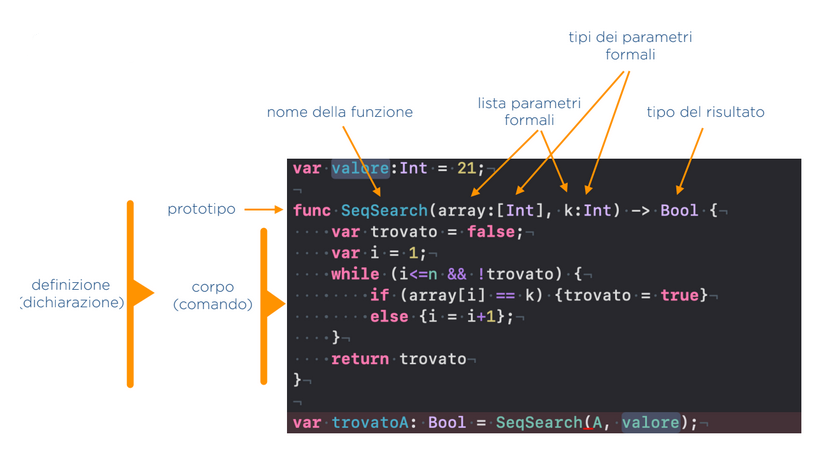
\includegraphics[width=13.5cm]{images/anatomia-funzione.png}
	\caption{}
\end{figure}
Il \textbf{compilatore} dovrà poi eseguire le seguenti verifiche:
\begin{itemize}
	\item il \textbf{numero} di parametri \emph{attuali} deve coincidere con quello dei parametri \emph{formali}
	\item i \textbf{nomi} dei parametri \emph{formali} devono essere tutti distinti
	\item i \textbf{tipi} degli \emph{attuali} e dei \emph{formali} nella stessa posizione devono essere uguali
	\item non ci devono essere \textbf{variabili libere} nel corpo della funzione che non possono essere legate
	\item deve esserci un \textbf{return statement} nel corpo della funzione
	\item il \textbf{tipo} dell'espressione nel \emph{return statement} deve coincidere con quello della dichiarazione
\end{itemize}
\subsubsection{Ambiente statico}
\begin{definition}[Principio di corrispondenza]
	Parti di programma che hanno effetti simili devono avere una sintassi simile. Facilità di apprendimento del linguaggio e di interpretazione dei programmi.
\end{definition}
\begin{definition}[Scoping statico]
	Le \textbf{variabili libere} nel corpo delle funzioni vengono legate a tempo di compilazione costruendo le \textbf{chiusure}.
\end{definition}
\begin{definition}[Chiusura]
	Ciò che viene registrato nell'\textbf{ambiente dinamico} al momento  dell'elaborazione della \textbf{dichiarazione} di funzione, associando al nome della funzione tutto ciò che sta alla sinistra.
\end{definition}
La dichiarazione di funzione genera nell’\textbf{ambiente dinamico} un legame tra il \textbf{nome della funzione} e una'\textbf{astrazione} che contiene tutte le informazioni necessarie ad eseguire la chiamata della funzione.
\begin{align}
	\centering
	[(nomeFunzione), \lambda(parametri formali) . {[(\textbf{variabili libere})], C}]
\end{align}
\begin{lstlisting}[language=Swift, caption=Esempio di scoping statico, mathescape=true]
	var COVID19:Bool = true;
	
	var mioCosto:Double = 100;
	var aliquota:Double = 21;
	
	// Chiusura
	// [(calcolaIVA, $\lambda$(let costo) . {[(aliquota, l2)]; return costo*aliquota/100})]
	
	func calcolaIVA(let costo:Double) -> Double {
		return costo*aliquota/100;
	}

	if (COVID19) {
		var aliquota:Double = 23;
		print(calcolaIVA(mioCosto));
	} else {
		print(calcolaIVA(mioCosto));
	}
\end{lstlisting}
\subsubsection{Ambiente dinamico}
Le \textbf{variabili libere} vengono legate a tempo di \textbf{esecuzione} quando vengono utilizzate. Nella chiusura della funzione registro solo il suo corpo al momento della dichiarazione.
\begin{lstlisting}[language=Swift, caption=Esempio di scoping dinamico, mathescape=true]
	var COVID19:Bool = true;
	
	var mioCosto:Double = 100;
	var aliquota:Double = 21;
	
	// Chiusura
	// [(calcolaIVA, $\lambda$(let costo) . {return costo*aliquota/100})]
	
	func calcolaIVA(let costo:Double) -> Double {
		return costo*aliquota/100;
	}
	
	if (COVID19) {
		var aliquota:Double = 23;
		print(calcolaIVA(mioCosto));
	} else {
		print(calcolaIVA(mioCosto));
	}
\end{lstlisting}
\color{red}\textbf{\title{IMPORTANTE}}\color{black}: la semantica statica ha senso solamente in presenza di uno \textbf{scoping statico}, il quale a differenza di quello dinamico ci garantisce la mancanza di errori. Di conseguenza in presenza dello \textbf{scoping dinamico} \color{red}MAI\color{black} verificare la correttezza sintattica.

\subsection{Passaggio dei parametri}
\subsubsection{Per valore}
Viene fatta una copia degli identificatori passati come parametri attuali tra le variabili locali del corpo della funzione. Non modifico il valore esterno di questi identificatori.

\subsubsection{Per indirizzo}